% =============================================================================
% Self-Evolution Protocol — Clean Minimal Arrow Design v3
% Key principle: MAX 2 arrows per anchor point, NO crossings.
%
% Layout:
%   Row 1:  BOOTSTRAP --> RUNTIME --> ADAPTIVE  (horizontal pipeline)
%   Row 2:  [Self-Evolution Engine] <--> [State]  (below center)
%
% Arrows (only 5 total, every one has a clear purpose):
%   ① Bootstrap -> Runtime       (forward pipeline)
%   ② Runtime -> Adaptive        (forward pipeline)
%   ③ All three cards -> Engine   (each drops straight down, no overlap)
%   ④ Engine <-> State           (horizontal, same row)
%   ⑤ Adaptive -> Bootstrap      (feedback U-loop along bottom edge)
% =============================================================================
\documentclass[tikz, border=10pt]{standalone}
\usepackage{tikz}
\usepackage{helvet}
\renewcommand{\familydefault}{\sfdefault}
\usetikzlibrary{arrows.meta, calc}

\definecolor{bootblue}{HTML}{0072B2}
\definecolor{learnorange}{HTML}{E69F00}
\definecolor{fallgreen}{HTML}{009E73}
\definecolor{ink}{HTML}{1A1A1A}
\definecolor{subink}{HTML}{555555}
\definecolor{softgray}{HTML}{E8E8E8}

\begin{document}
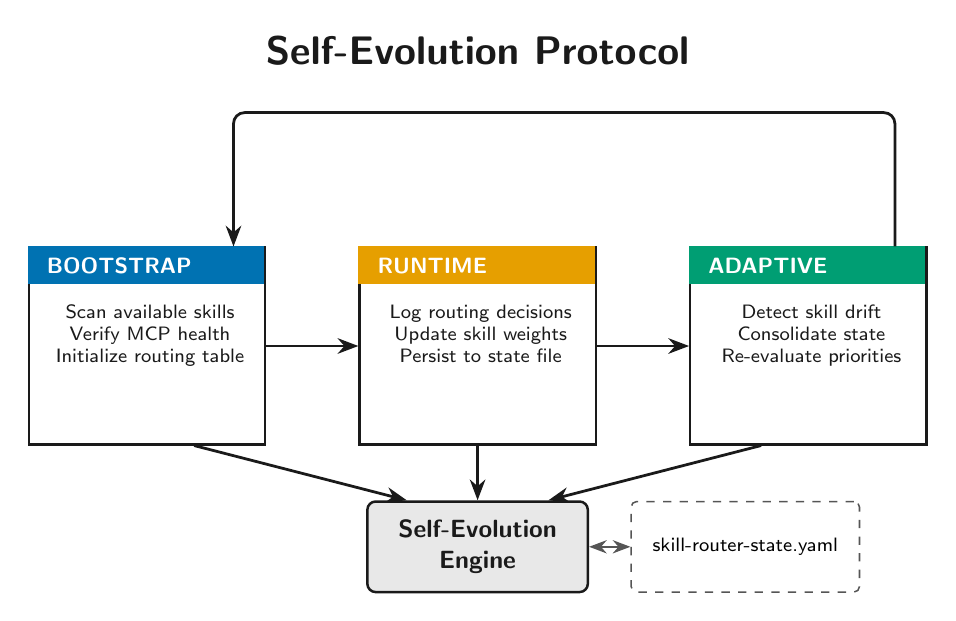
\begin{tikzpicture}[
    >=Stealth,
    arr/.style={->, line width=1.0pt, ink, rounded corners=4pt},
    bi/.style={<->, line width=0.75pt, subink},
    every node/.style={font=\sffamily, align=center},
    % Process card
    pcard/.style={rectangle, draw=ink, line width=0.8pt, fill=white,
                  minimum width=3.0cm, minimum height=2.5cm, align=left,
                  inner sep=7pt},
    % Small box
    sbox/.style={rectangle, rounded corners=3pt, draw=ink, line width=0.9pt,
                 minimum width=2.8cm, minimum height=1.15cm, align=center,
                 font=\small\bfseries, inner sep=6pt},
    stbox/.style={rectangle, rounded corners=2pt, draw=subink, line width=0.55pt,
                  dashed, fill=white, minimum width=2.9cm, minimum height=1.15cm,
                  font=\scriptsize, align=center, inner sep=5pt}
]

% ========== Title ==========
\node[font=\Large\bfseries, text=ink] at (0, 5.6) {Self-Evolution Protocol};

% ========== ROW 1: Three cards ==========
% --- Bootstrap ---
\node[pcard] at (-4.2, 1.85) (boot) {};
\fill[bootblue] (boot.north west) rectangle ([xshift=3.0cm, yshift=-0.48cm]boot.north west);
\node[font=\bfseries\footnotesize, text=white, anchor=west]
    at ([xshift=0.12cm, yshift=-0.24cm]boot.north west) {BOOTSTRAP};
\node[font=\scriptsize, text=ink, anchor=north west, text width=2.7cm]
    at ([xshift=0.08cm, yshift=-0.62cm]boot.north west)
    {Scan available skills\\Verify MCP health\\Initialize routing table};

% --- Runtime ---
\node[pcard] at (0, 1.85) (learn) {};
\fill[learnorange] (learn.north west) rectangle ([xshift=3.0cm, yshift=-0.48cm]learn.north west);
\node[font=\bfseries\footnotesize, text=white, anchor=west]
    at ([xshift=0.12cm, yshift=-0.24cm]learn.north west) {RUNTIME};
\node[font=\scriptsize, text=ink, anchor=north west, text width=2.7cm]
    at ([xshift=0.08cm, yshift=-0.62cm]learn.north west)
    {Log routing decisions\\Update skill weights\\Persist to state file};

% --- Adaptive ---
\node[pcard] at (4.2, 1.85) (fall) {};
\fill[fallgreen] (fall.north west) rectangle ([xshift=3.0cm, yshift=-0.48cm]fall.north west);
\node[font=\bfseries\footnotesize, text=white, anchor=west]
    at ([xshift=0.12cm, yshift=-0.24cm]fall.north west) {ADAPTIVE};
\node[font=\scriptsize, text=ink, anchor=north west, text width=2.7cm]
    at ([xshift=0.08cm, yshift=-0.62cm]fall.north west)
    {Detect skill drift\\Consolidate state\\Re-evaluate priorities};

% ========== ROW 2: Engine + State ==========
\node[sbox, fill=softgray, text=ink] at (0, -0.7) (cen) {Self-Evolution\\Engine};

\node[stbox] at (3.4, -0.7) (state) {skill-router-state.yaml};

% ========== ARROWS (5 total, carefully placed) ==========

% --- ①+② Forward pipeline: Bootstrap -> Runtime -> Adaptive ---
\draw[arr] (boot.east) -- (learn.west);
\draw[arr] (learn.east) -- (fall.west);

% --- ③ Cards -> Engine: each card has exactly ONE downward arrow ---
% Bootstrap -> Engine (from south-right of boot, angled down to engine's north-west)
\draw[arr] ($(boot.south) + (0.6, 0)$) -- ($(cen.north) + (-0.9, 0)$);
% Runtime -> Engine (straight down, centered)
\draw[arr] (learn.south) -- (cen.north);
% Adaptive -> Engine (from south-left of fall, angled down to engine's north-east)
\draw[arr] ($(fall.south) + (-0.6, 0)$) -- ($(cen.north) + (0.9, 0)$);

% --- ④ Engine <-> State (horizontal, no overlap with anything) ---
\draw[bi] (cen.east) -- (state.west);

% --- ⑤ Feedback loop: Adaptive -> Bootstrap (U-shaped along TOP outer boundary) ---
% Path: fall outer-north -> up (well above cards) -> left -> down into boot outer-north
\draw[arr] ($(fall.north) + (1.1, 0)$) -- ++(0, 1.7) -| ($(boot.north) + (1.1, 0)$);

% --- Legend removed (arrow types are self-evident) ---

\end{tikzpicture}
\end{document}
